% USENIX-style two-column paper
% To use the official USENIX template, replace this preamble with:
%   \documentclass[letterpaper,twocolumn,10pt]{article}
%   \usepackage{usenix2019_v3}
% Download from: https://www.usenix.org/conferences/author-resources/paper-templates

\documentclass[letterpaper,twocolumn,10pt]{article}

% ─── Packages ────────────────────────────────────────────────
\usepackage[utf8]{inputenc}
\usepackage[T1]{fontenc}
\usepackage{times}              % USENIX uses Times font
\usepackage{mathptmx}           % Times math
\usepackage[margin=1in]{geometry}
\usepackage{graphicx}
\usepackage{booktabs}
\usepackage{amsmath,amssymb}
\usepackage{hyperref}
\usepackage{xcolor}
\usepackage{enumitem}
\usepackage{caption}
\usepackage{subcaption}
\usepackage[numbers]{natbib}
\usepackage{balance}            % Balance last page columns

% ─── Hyperlink styling ───────────────────────────────────────
\hypersetup{
  colorlinks=true,
  linkcolor=blue!60!black,
  citecolor=blue!60!black,
  urlcolor=blue!60!black,
}

% ─── Tight lists ─────────────────────────────────────────────
\setlist{nosep,leftmargin=1.5em}

% ─── Title ───────────────────────────────────────────────────
\title{\Large \bf When Does Value-Density Eviction Help?\\
A Workload-Dependent Analysis of KV Cache Eviction for LLM Serving}

\author{
  {\rm Aditya Lawankar} \\
  % Institution / Affiliation
}

\date{}

\begin{document}
\maketitle

% ═════════════════════════════════════════════════════════════
\begin{abstract}
Large Language Model serving is bottlenecked by memory capacity for Key-Value (KV) caches. Multi-turn conversations and long-context workloads force frequent cache eviction and costly recomputation (the ``cold-start'' problem). We build a three-tier KV cache persistence system and evaluate learned eviction policies across three workload profiles. Our investigation yields three findings: (1)~binary classification eviction underperforms LRU by 16 percentage points due to a Knapsack formulation mismatch; (2)~static Fractional Knapsack optimization collapses cache cardinality in dynamic systems governed by Little's Law, dropping hit rates by 23 points on heavy-tailed workloads; and (3)~despite a lower hit rate, our learned policy achieves \$68/day higher GPU savings than LRU on power-user workloads by disproportionately retaining expensive-to-recompute sessions. We validate end-to-end with TinyLlama-1.1B, demonstrating 48$\times$ TTFT improvement with semantically lossless cache restoration. We propose Space-Time density as the theoretically grounded objective for next-generation eviction policy design.
\end{abstract}

% CCS / Index terms
\vspace{0.5em}
\noindent\textbf{Keywords:} Cache Replacement Algorithms, LLM Inference, Tiered Storage, KV Cache, ML Systems

% ═════════════════════════════════════════════════════════════
\section{Introduction}

The cold-start problem in LLM inference occurs when a user resumes a session whose KV cache has been evicted from VRAM. The system must reprocess the entire prompt history through the transformer's prefill phase, wasting compute and increasing time-to-first-token (TTFT). Existing systems like vLLM~\cite{kwon2023pagedattention} rely on reactive LRU eviction, discarding valuable context without regard to recompute cost.

We explore tiered persistence (VRAM $\to$ NVMe $\to$ Object Storage) combined with predictive eviction. By proactively migrating idle sessions to cheaper tiers, we hypothesized we could improve cache hit rates. Our investigation uncovered fundamental limitations in applying textbook optimization to dynamic systems, yielding insights generalizable beyond KV caching.

This paper makes the following contributions:
\begin{enumerate}
  \item A \textbf{three-tier KV cache persistence system} with pluggable eviction backends supporting LRU, heuristic, ML-based, and value-density policies.
  \item An \textbf{empirical demonstration that binary classification eviction fails} under constrained capacity due to a Knapsack formulation mismatch, underperforming LRU by 16 percentage points.
  \item The discovery that \textbf{static Fractional Knapsack optimization collapses cache cardinality} in dynamic systems governed by Little's Law.
  \item Evidence that \textbf{learned policies can maximize cache value} (\$/Day) rather than hit count on high-variance workloads, outperforming LRU by \$68/day despite lower hit rate.
  \item A \textbf{Space-Time density framework} as the theoretically grounded objective for future eviction policy design.
\end{enumerate}

% ═════════════════════════════════════════════════════════════
\section{Background}

\subsection{Self-Attention and the KV Cache}
The self-attention mechanism in transformer-based LLMs attends to all previous tokens. The prefill phase grows quadratically $O(N^2)$ with sequence length $N$, while KV cache memory grows linearly $O(N)$. Inference engines cache key and value tensors in VRAM; however, VRAM is severely constrained, necessitating eviction policies when multiple sessions compete.

\subsection{B\'{e}l\'{a}dy's Algorithm}
The provably optimal offline eviction policy~\cite{belady1966replacement} evicts the item whose next access occurs furthest in the future: $\arg\max_{i} \text{next\_access}(i)$. For uniform-size, uniform-cost items, LRU is an effective online proxy by assuming temporal locality.

\subsection{Weighted Caching}
When items have varying sizes and costs, the uniform assumption fails. The problem maps to a dynamic Fractional Knapsack. As formalized by Young~\cite{young1994caching}, optimal eviction must maximize value density per byte. In KV caching, ``value'' is the quadratic GPU compute saved by avoiding a cold-start prefill, and ``weight'' is the linear VRAM consumed.

% ═════════════════════════════════════════════════════════════
\section{Related Work}

PagedAttention~\cite{kwon2023pagedattention} partitions the KV cache into fixed-size blocks, eliminating fragmentation and enabling memory sharing. vLLM manages VRAM dynamically but relies on reactive LRU eviction. CachedAttention~\cite{gim2024cachedattention} supports cross-request caching at the attention layer, though its focus is architectural integration rather than learned eviction policies.

LMCache~\cite{zhong2024lmcache} and CacheBlend~\cite{yao2024cacheblend} focus on cross-request prefix sharing---caching system prompts shared across users. Our work targets single-session persistence: saving user-specific conversational state over long time horizons, where the challenge is predicting which sessions will return.

Mooncake~\cite{qin2025mooncake} proposes a disaggregated KV cache architecture using a tiered hierarchy across nodes. Our work shares the tiered storage motivation but targets the algorithmic eviction policy layer. Where Mooncake asks ``how do we distribute cache across a cluster?'', we ask ``which entries should we keep when capacity is constrained?''

% ═════════════════════════════════════════════════════════════
\section{System Design}

Our architecture introduces a \texttt{TieredCacheManager} orchestrating three storage tiers:

\begin{enumerate}
  \item \textbf{Hot Tier (VRAM):} In-memory storage. ${\sim}0.1$ms latency, 50MB capacity.
  \item \textbf{Warm Tier (NVMe SSD):} Filesystem-backed with memory-mapped reads for files $>$10MB. ${\sim}10$ms latency, 150MB capacity.
  \item \textbf{Cold Tier (S3/MinIO):} Object storage with Zstandard compression. ${\sim}100$ms latency, 300MB capacity.
\end{enumerate}

The system exposes three operations: \texttt{save} (serialize and write to hot tier with cascading eviction), \texttt{load} (search tiers in order, deserialize on hit), and \texttt{demote}/\texttt{promote} (explicit tier migration).

\begin{table}[t]
\centering
\caption{Tier transition pipeline}
\label{tab:transitions}
\small
\begin{tabular}{@{}llll@{}}
\toprule
Transition & Serialization & Compression & Rationale \\
\midrule
Hot $\to$ Warm & Raw Binary & None & Minimize latency \\
Warm $\to$ Cold & Raw Binary & Zstd (L3) & Optimize capacity \\
Cold $\to$ Warm & Raw Binary & Zstd decomp. & Async prefetch \\
\bottomrule
\end{tabular}
\end{table}

Serialization uses a custom binary format with a 64-byte header (magic bytes, version, layer count, tensor dimensions, dtype) followed by packed FP16 tensor data. This is 3--5$\times$ faster than \texttt{safetensors} for hot$\leftrightarrow$warm transfers.

% ═════════════════════════════════════════════════════════════
\section{Eviction Policy V1: Binary Classification}

Our initial approach formulated eviction as supervised ML: predict $P(\text{resume})$ that a session will be accessed again within 1~hour. We engineered 9~features capturing temporal patterns, access behavior, user history, and session characteristics. We trained Logistic Regression and Gradient Boosted Trees (GBT) on 10,000 synthetic trace events (80/20 split). GBT achieved marginally higher accuracy but introduced prohibitive P95 latency (${\sim}359$ms vs ${\sim}100$ms for Logistic Regression) and is excluded from the main evaluation.

\textbf{Negative Result:} Under enterprise load with 30MB capacity, Logistic~V1 achieved only \textbf{39.13\%} hit rate---significantly worse than LRU's \textbf{55.25\%}.

% ═════════════════════════════════════════════════════════════
\section{Failure Analysis}

This exposed a fundamental flaw: \textbf{eviction under capacity constraints is not a classification problem; it is a Knapsack variant.} LRU accidentally approximated correct behavior by rotating entries uniformly. Our ML models confidently kept large ``high probability'' sessions that choked capacity, forcing out dozens of smaller entries. The binary criterion $\min P(\text{resume})$ ignores both entry size and variable recompute cost.

% ═════════════════════════════════════════════════════════════
\section{Eviction Policy V2: Value-Density Maximization}

We reformulated the objective based on weighted caching theory:
\begin{equation}
  \text{Value Density} = \frac{P(\text{resume}) \times \text{RecomputeCost}(N)}{\text{SizeBytes}(N)}
  \label{eq:vd}
\end{equation}

Because prefill scales $O(N^2)$ but memory scales $O(N)$, longer contexts have exponentially higher value density. We also implemented an \textbf{Admission Control Gate}: sessions below a value-density threshold are denied entry to the warm tier.

\subsection{Space-Time Density: Why Static Knapsack Fails}

Our evaluation revealed that static value-density collapses in practice (\S\ref{sec:eval}). A cache is not a static knapsack---it is a dynamic system governed by Little's Law. Each entry occupies \emph{space over time}. The correct objective must account for expected sojourn time $\mathbb{E}[\Delta t]$:
\begin{equation}
  \text{Space-Time Density} = \frac{P(\text{resume}) \times \text{RecomputeCost}(N)}{\text{Size}(N) \times \mathbb{E}[\Delta t]}
  \label{eq:std}
\end{equation}

Under Little's Law, $L = \lambda \times W$, where $L$ is steady-state items, $\lambda$ is arrival rate, and $W$ is average sojourn time. Maximizing $\text{Value}/\text{Byte}$ without bounding $W$ allows large sessions to accumulate unbounded sojourn time, reducing $L$ (cardinality) and collapsing hit rates. This formulation provides the theoretical foundation for a V3 policy.

% ═════════════════════════════════════════════════════════════
\section{Experimental Setup}

We evaluated eviction policies using a synthetic workload simulator with three profiles via Poisson arrivals and Log-normal token distributions:
\begin{itemize}
  \item \textbf{Casual:} 50/hr arrival, $\mu{=}512$, $\sigma{=}0.8$, low return probability.
  \item \textbf{Enterprise:} 200/hr, $\mu{=}2048$, $\sigma{=}0.5$, high return probability.
  \item \textbf{Power User:} 80/hr, $\mu{=}8192$, $\sigma{=}1.2$, medium return probability.
\end{itemize}

\textbf{Model Configuration.} KV cache sizes are computed using a toy configuration (2~layers, 2~heads, head dimension~32, FP16). A production model (e.g., Llama-2 7B: 32~layers, 32~heads, head dimension~128) would increase sizes by ${\sim}256\times$, shifting absolute capacity dynamics but not relative policy comparisons.

\textbf{Simulation.} 6-hour continuous window; token counts clamped to 8,192 to preserve heavy-tailed distributions, yielding a $498\times$ spread in quadratic recompute costs.

\textbf{Capacity.} 500MB total (50MB hot + 150MB warm + 300MB cold), relaxed from 30MB used during V1 debugging.

\textbf{GPU Savings.} Computed by summing exact $O(N^2)$ recompute cost of each hit session, rather than multiplying hit rate by average cost.

\textbf{Confidence Intervals.} 95\% CIs via bootstrap resampling (1,000 iterations).

% ═════════════════════════════════════════════════════════════
\section{Comparative Evaluation}
\label{sec:eval}

We evaluated 5 policies across 3 workloads. The casual workload achieved 100\% hit rate at 500MB---the cache was never constrained---so we focus on the two workloads where eviction pressure forces policy differentiation.

\begin{table}[t]
\centering
\caption{Policy comparison across workloads (500MB, 6hr simulation)}
\label{tab:results}
\small
\begin{tabular}{@{}llrrrr@{}}
\toprule
Policy & Workload & Hit\% & 95\% CI & P95 & \$/Day \\
\midrule
LRU        & Enterprise & 97.09 & [96.2, 97.9] & 188ms & \$1,038 \\
Heuristic  & Enterprise & 61.81 & [59.2, 64.3] & 171ms & \$661  \\
Logistic   & Enterprise & 79.55 & [77.5, 81.5] & 325ms & \$850  \\
ValDensity & Enterprise & 70.14 & [67.8, 72.5] & 362ms & \$750  \\
ValDens+AC & Enterprise & 70.14 & [67.8, 72.5] & 365ms & \$750  \\
\midrule
LRU        & Power User & 92.64 & [89.2, 96.1] & 135ms & \$3,447 \\
Heuristic  & Power User & 69.26 & [63.2, 74.9] & 105ms & \$2,832 \\
Logistic   & Power User & 87.45 & [82.7, 91.3] & 191ms & \$3,515 \\
ValDensity & Power User & 69.26 & [63.6, 75.8] & 184ms & \$3,303 \\
ValDens+AC & Power User & 69.26 & [63.6, 75.8] & 186ms & \$3,303 \\
\bottomrule
\end{tabular}
\end{table}

\begin{figure}[t]
  \centering
  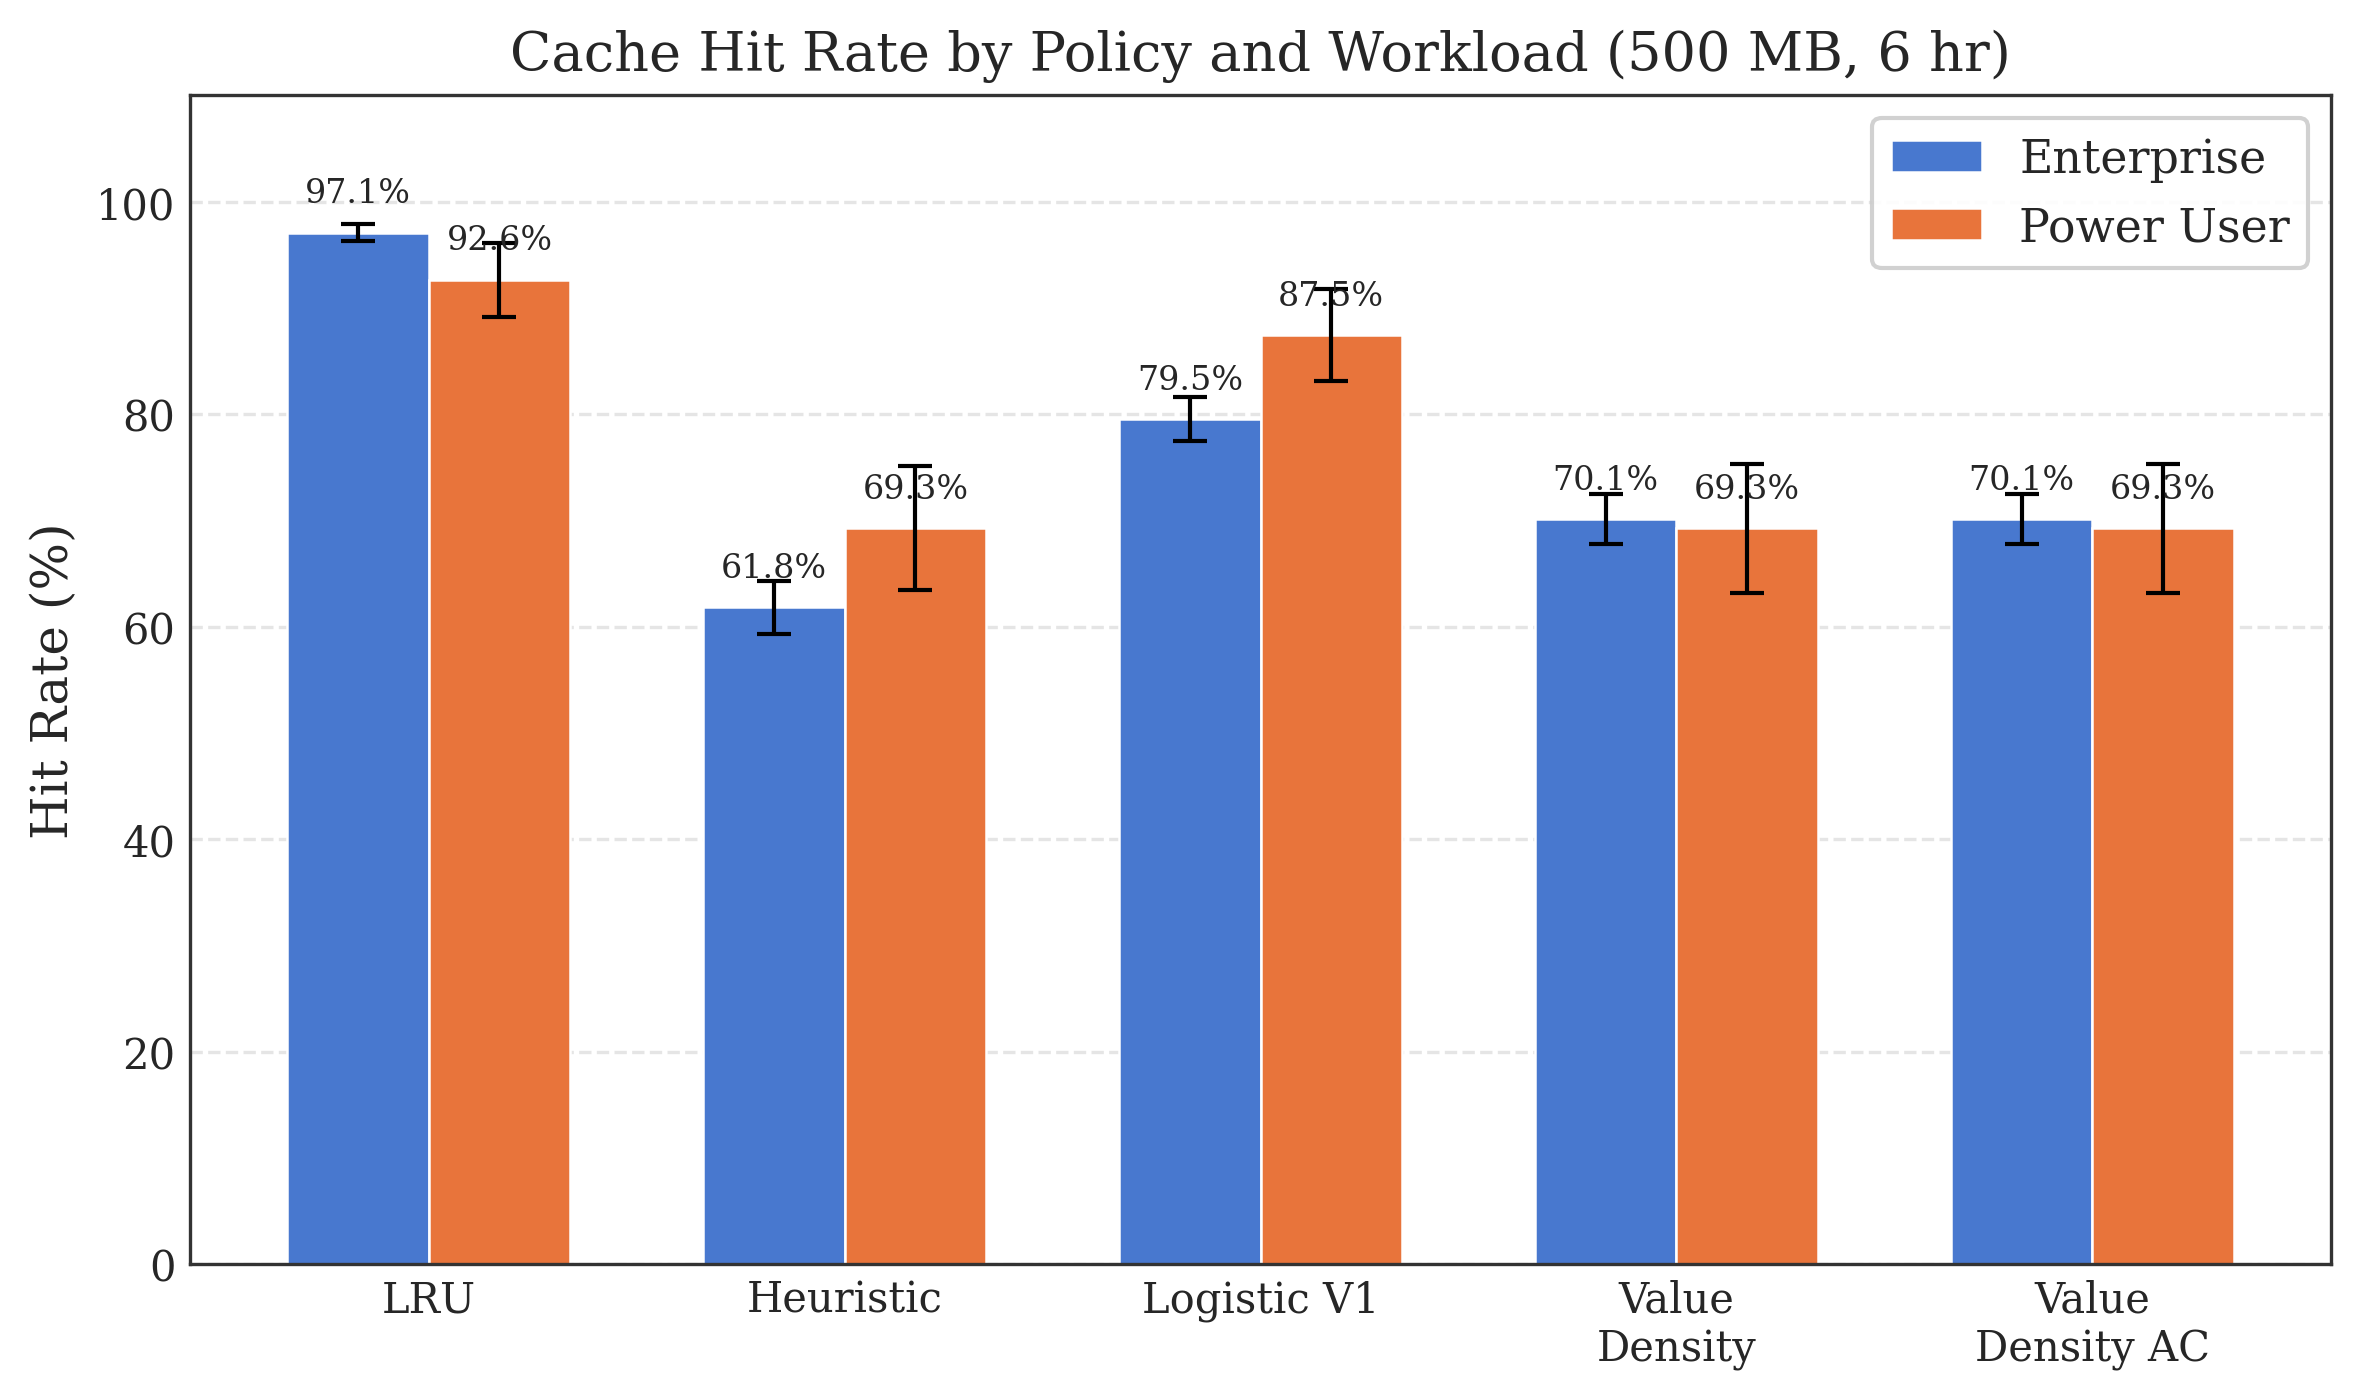
\includegraphics[width=\columnwidth]{figures/figure1_hit_rate.png}
  \caption{Cache hit rate by policy and workload with 95\% CI error bars. LRU dominates on enterprise; all policies struggle on power-user.}
  \label{fig:hitrate}
\end{figure}

\begin{figure}[t]
  \centering
  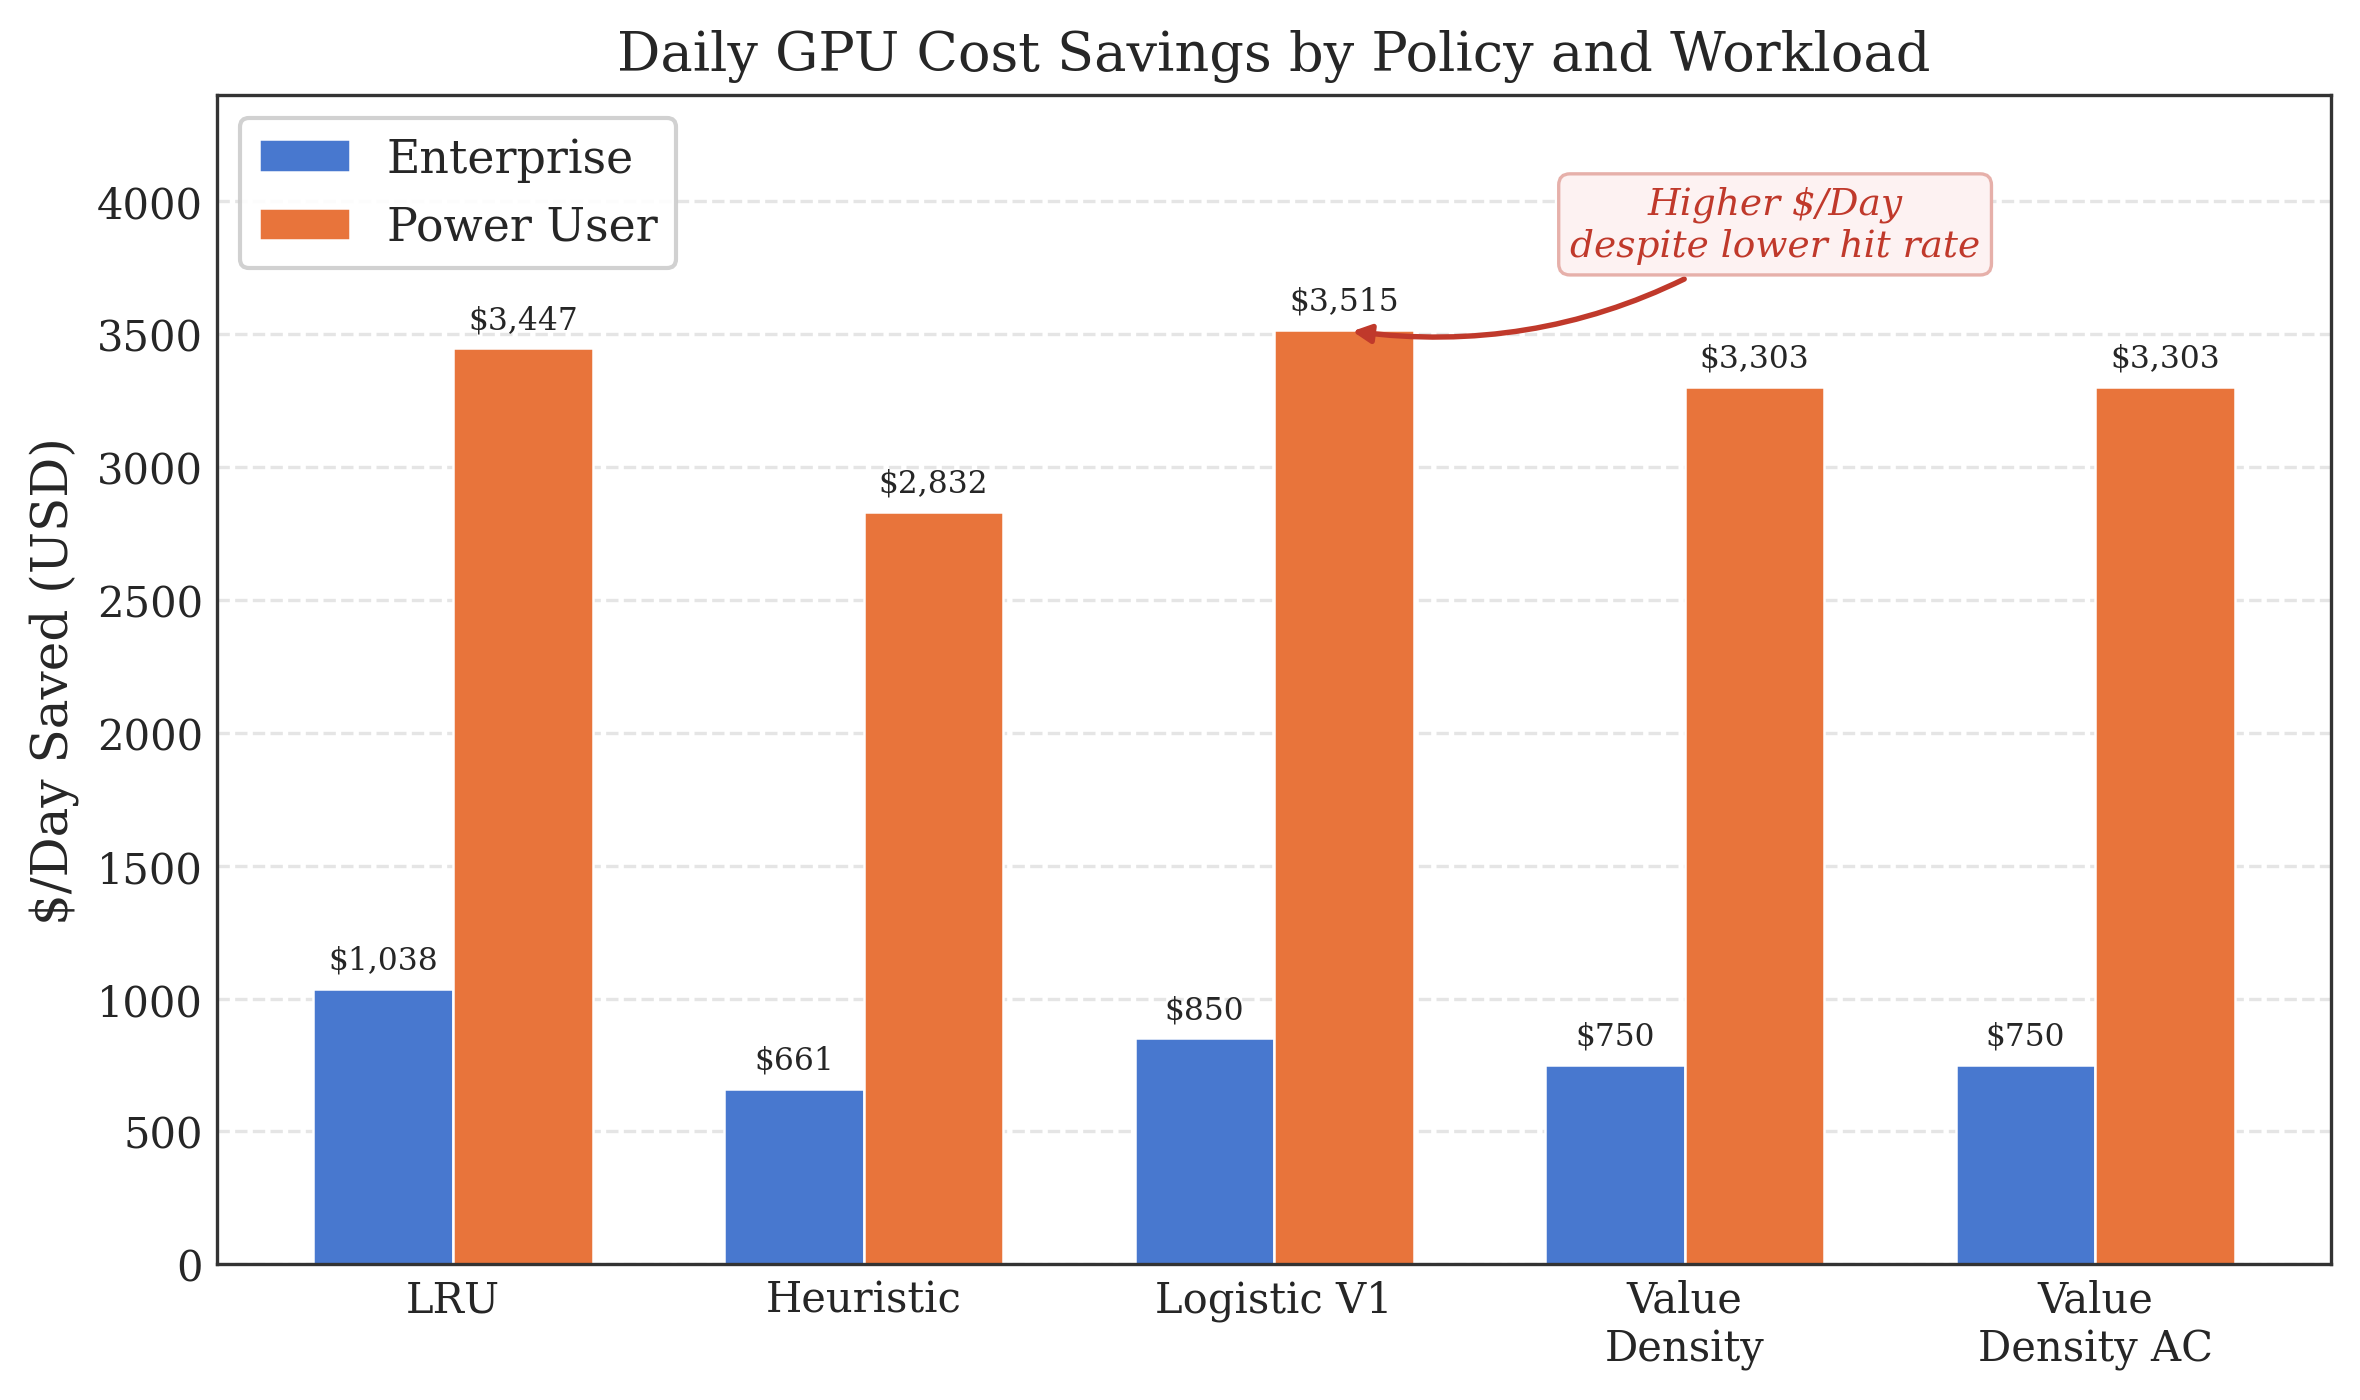
\includegraphics[width=\columnwidth]{figures/figure2_cost_savings.png}
  \caption{Daily GPU cost savings. Despite lower hit rate, Logistic~V1 exceeds LRU by \$68/day on power-user workloads.}
  \label{fig:savings}
\end{figure}

\subsection{Why Knapsack Fails in Dynamic Caching}

V2 Value Density plummeted to 69.26\% hit rate on power-user, underperforming LRU (92.64\%) and Logistic~V1 (87.45\%). The Fractional Knapsack algorithm is optimal for \emph{static} packing, but a cache is \emph{dynamic} under Little's Law. By maximizing value density, V2 retained massive 8,192-token sessions, dropping cache cardinality from ${\sim}250$ to ${\sim}15$. The cache was starved, and large sessions were eventually evicted before their high $P(\text{resume})$ could materialize into hits.

Admission control (V2+AC) produced no improvement at 500MB---under sustained load, the cache operates at near-full utilization regardless of filtering.

\begin{figure}[t]
  \centering
  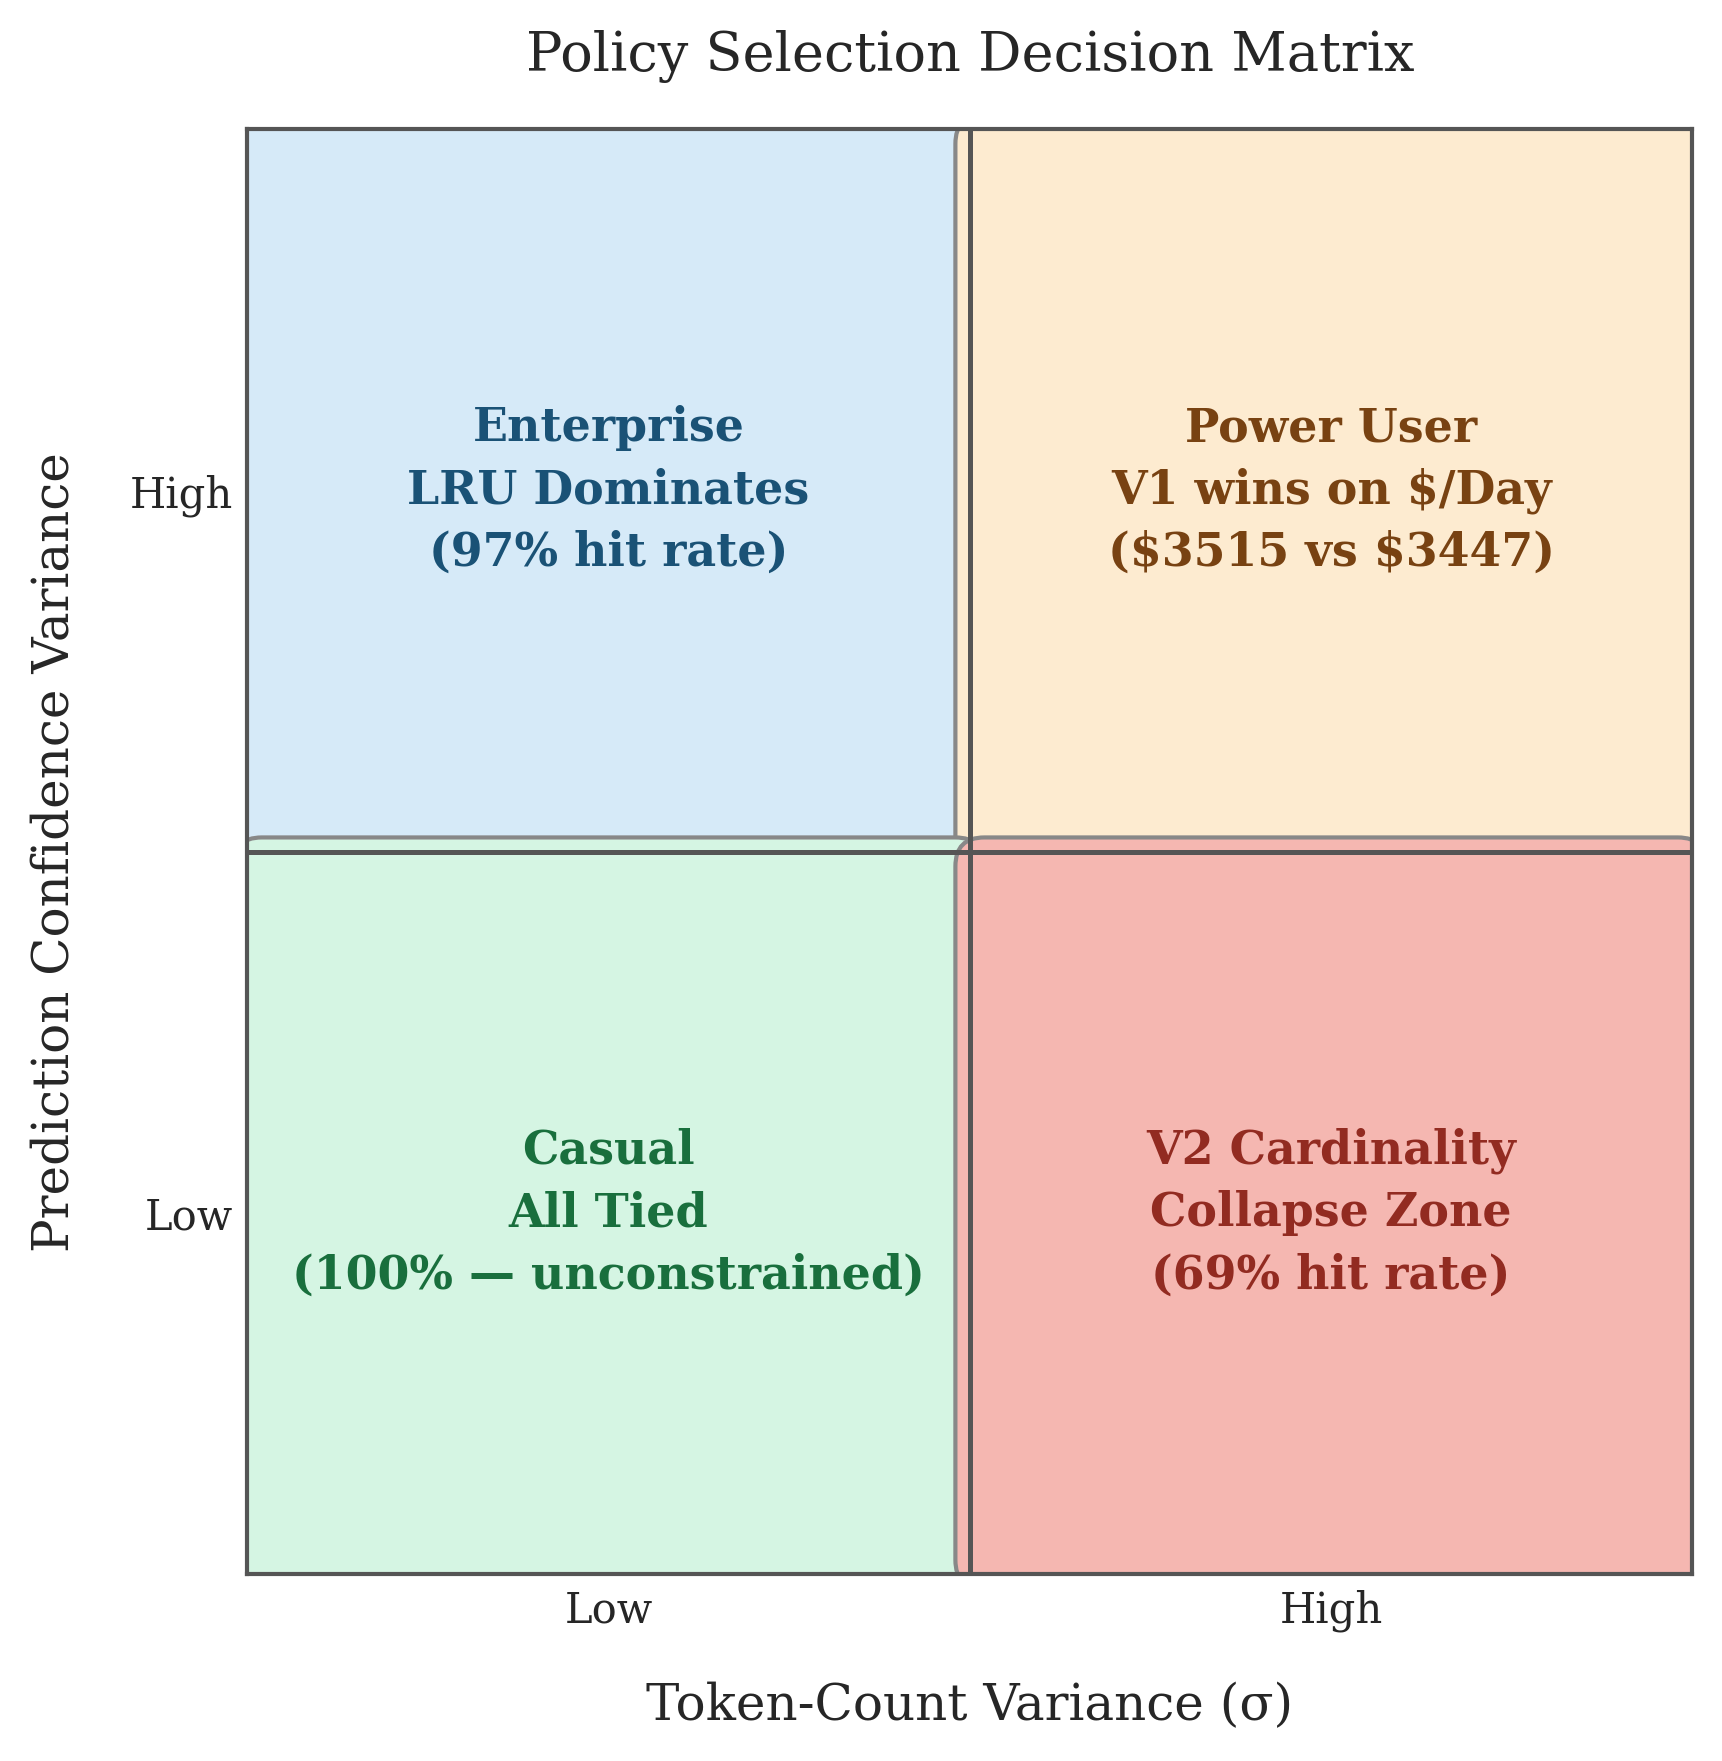
\includegraphics[width=\columnwidth]{figures/figure3_failure_modes.png}
  \caption{Policy selection decision matrix mapping failure modes by workload variance characteristics.}
  \label{fig:failuremodes}
\end{figure}

\subsection{Hit Rate Is the Wrong Metric}

Despite \emph{lower} hit rate than LRU (87.45\% vs 92.64\%), Logistic~V1 delivers \emph{higher} GPU savings (\$3,515 vs \$3,447)---a \$68/day difference. LRU retains sessions uniformly by recency; Logistic~V1 disproportionately retains long-context, high-return sessions where each hit saves \$20 of GPU compute rather than \$0.50. This \$68/day advantage corresponds to 80~power users/hr over 24~hours; at production scale, the gap compounds proportionally.

\textbf{The correct optimization target for learned cache policies is not hit rate---it is expected cache value.}

% ═════════════════════════════════════════════════════════════
\section{Prototype Validation: TinyLlama}

To validate with a real transformer, we integrated our \texttt{TieredCacheManager} with TinyLlama-1.1B-Chat~(22~layers, 32~Q-heads, 4~KV-heads via GQA, head\_dim=64) on CPU.

\textbf{GQA Compatibility.} Modern models use Grouped Query Attention where KV heads (4) differ from query heads (32). Our serialization must use \texttt{num\_key\_value\_heads} for tensor dimensions---a critical detail for production deployment.

\begin{table}[t]
\centering
\caption{TinyLlama integration results (598-token prompt, CPU)}
\label{tab:tinyllama}
\small
\begin{tabular}{@{}lrrr@{}}
\toprule
Metric & Trial 1 & Trial 2 & Average \\
\midrule
Cold-start TTFT       & 11,804ms & 11,449ms & 11,627ms \\
Warm-start TTFT       & 239ms    & 243ms    & 241ms    \\
TTFT speedup          & 49.4$\times$ & 47.1$\times$ & 48.3$\times$ \\
E2E speedup (30 tok.) & 1.80$\times$ & 1.69$\times$ & 1.75$\times$ \\
Cache size (FP16)     & 13,156 KB & 13,156 KB & 13,156 KB \\
Save latency          & 55ms     & 57ms     & 56ms     \\
Load latency          & 4ms      & 5ms      & 4.5ms    \\
Semantic match        & \checkmark & \checkmark & 100\%  \\
\bottomrule
\end{tabular}
\end{table}

Warm-start TTFT of \textbf{241ms} versus cold-start 11,627ms represents a \textbf{48$\times$ improvement}. End-to-end speedup is 1.75$\times$ because decode-phase speed is independent of cache state. Greedy-decoded output was byte-identical, confirming FP16 quantization introduces no degradation.

\textbf{Cost Model Calibration.} Our simulation cost model (A100 GPU, \$2.50/hr) predicted 57,747ms for 598-token prefill versus actual 11,627ms on CPU---expected since model parameters must be calibrated per hardware. Relative policy comparisons remain valid.

% ═════════════════════════════════════════════════════════════
\section{Discussion \& Future Work}

\textbf{The Metric Mismatch.} Hit rate assumes uniform item value. In KV caching with quadratic recompute costs, this is catastrophically wrong. Production systems must adopt value-weighted metrics (e.g., GPU-seconds saved per decision).

\textbf{Decision Framework.} (1)~Uniform workloads ($\sigma{=}0.5$): LRU dominates---ML overhead is unjustified. (2)~High-variance ($\sigma{=}1.2$): learned policies outperform \emph{by value}; evaluate by \$/Day. (3)~Extreme heterogeneity: static Value-Density is counterproductive; await Space-Time implementations.

\textbf{Limitations.} (1)~Synthetic workloads may miss real user correlations. (2)~CPU-only TinyLlama validation omits GPU-specific effects (CUDA fragmentation, PCIe overhead). (3)~Simulated tier latencies underestimate production I/O. (4)~Scaling to 70B models shifts absolute capacity dynamics.

\textbf{V3 Path.} Space-Time density (Eq.~\ref{eq:std}) provides the V3 foundation. $\mathbb{E}[\Delta t]$ can be estimated via exponential smoothing with ${\sim}2$hr half-life. The key challenge is continuous re-scoring as entries age, requiring periodic sweeps rather than one-shot decisions. Integrating with admission control can prevent cardinality collapse while preserving $O(N^2)$ cost awareness.

% ═════════════════════════════════════════════════════════════
\section{Conclusion}

We presented a three-tier KV cache persistence system and evaluated five eviction policies across three workloads, validated end-to-end with TinyLlama-1.1B. Our investigation yielded three key insights: (1)~binary classification fails due to Knapsack mismatch; (2)~static Fractional Knapsack collapses cardinality under Little's Law; (3)~learned policies maximize cache \emph{value} over \emph{count}, outperforming LRU by \$68/day despite lower hit rate. Prototype validation demonstrates 48$\times$ TTFT improvement with lossless restoration. We propose Space-Time density as the objective for next-generation eviction design.

% ═════════════════════════════════════════════════════════════
\balance
\bibliographystyle{plainnat}
\bibliography{references}

\end{document}
